\documentclass[smaller]{beamer}
\usepackage{beamerarticle}
\mode<presentation> {
  \usetheme[width=80pt]{Berkeley}
  \useinnertheme{circles}
  \usecolortheme{sidebartab}
  \setbeamercolor{structure}{fg=blue}
  % or ...

%  \setbeamercovered{transparent}
  % or whatever (possibly just delete it)
}

%\usepackage[russian]{babel}
%\usepackage[cp1251]{inputenc}
%\usepackage[utf8]{inputenc}
%\usepackage{listings}
%\usepackage[pdftex,unicode]{hyperref}
%\usepackage[english]{babel}
\usefonttheme{serif}
% Or whatever. Note that the encoding and the font should match. If T1
% does not look nice, try deleting the line with the fontenc.


\title{Fuzzy Patterns} % (optional, use only with long paper titles)

\author % (optional, use only with lots of authors)
{V.\,V.\,Vishnevskiy\inst{1}}
\institute[Moscow State University] % (optional, but mostly needed)
{
  \inst{1}
  Moscow State University
}

\date[Patterns] % (optional, should be abbreviation of conference name)
{}
% - Either use conference name or its abbreviation.
% - Not really informative to the audience, more for people (including
%   yourself) who are reading the slides online

\AtBeginSubsection[] {
  \begin{frame}<beamer>
    \frametitle{Plan}
    \tableofcontents[currentsection,currentsubsection]
  \end{frame}
}
\begin{document}

\begin{frame}
  \titlepage
\end{frame}

\begin{frame}
  \frametitle{Plan}
  \tableofcontents
  % You might wish to add the option [pausesections]
\end{frame}



\section{Introduction}

\begin{frame}	
  \frametitle{Basic notions}
\begin{itemize}
  \item Behavioral events(acts): $A,B,C,D\dots$
  \item Each event occurs at certain time moments: $t_{A_1},\dots,t_{A_N}$. 
  \item Pattern is a chain of events, that occur one after another quite often.
\end{itemize}

\begin{left}
\begin{tabular}[t]{p{12em}|p{12em}}
    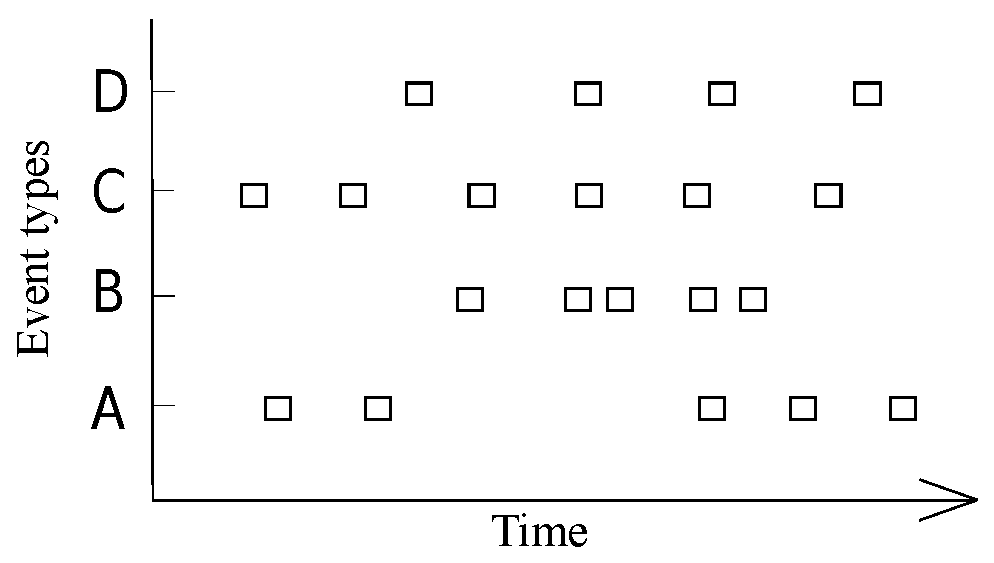
\includegraphics[scale=0.25]{NEWTS.eps} & 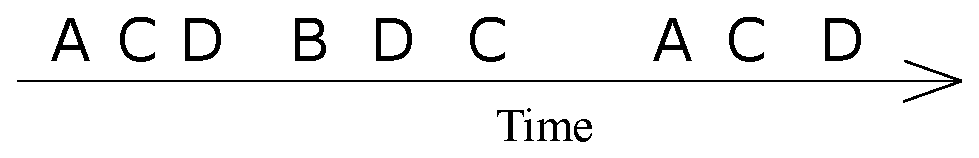
\includegraphics[scale=0.25]{TSNEW2.eps}\\
\end{tabular}
\end{left}


\end{frame}

\subsection{ T-Patterns}
\begin{frame}
  \frametitle{T-Patterns data types}
\begin{itemize}
  \item Events are joined with critical intervals. $A[d_1,d_2]B$.
  \item Critical interval relation means that event $B$ occurs after 
	event $A$ in time span $[t_A + d_1, t_A + d_2 ]$, more often than usual.
\end{itemize}
  \begin{center}
      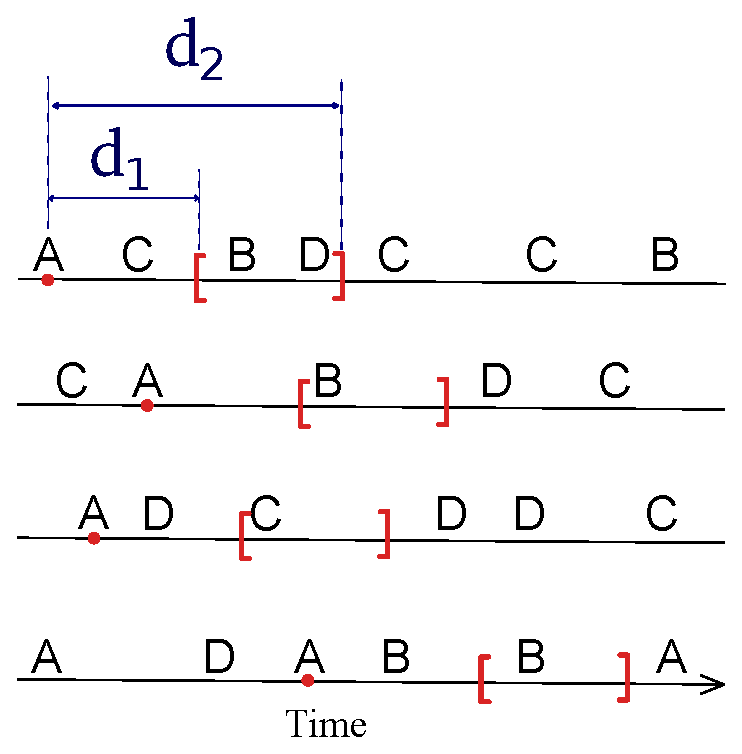
\includegraphics[scale=0.42]{TSCI.eps}
  \end{center}
\end{frame}

\begin{frame}
  \frametitle{T-Patterns detection procedure}
  Repeat while new patterns are detected:
\begin{itemize}
  \item For each two patterns try to join them with 
	critical interval relation.
  \item Delete duplicate and incomplete patterns.
\end{itemize}
\end{frame}


% \begin{frame}
%   \frametitle{T-Patterns drawbacks}
% \begin{itemize}
%   \item Sensitive to noise.
%   \item Crisp patterns.
% \end{itemize}
% \end{frame}

\section{Fuzzy Patterns}
\begin{frame}
  \frametitle{Proposed method}
\begin{itemize}
  \item Probabilistic pattern representation.
  \item Same iterative process.
\end{itemize}
\end{frame}

\begin{frame}
  \frametitle{Pattern representation }
\begin{itemize}
  \item Pattern consists of events.
  \item Each event in pattern characterized by mean shift and variance from 
	previous event.
  \item $P=A[0,\sigma_A]B[\mu_B,\sigma_B]C[\mu_C,\sigma_C]$.
\end{itemize}
\begin{center}
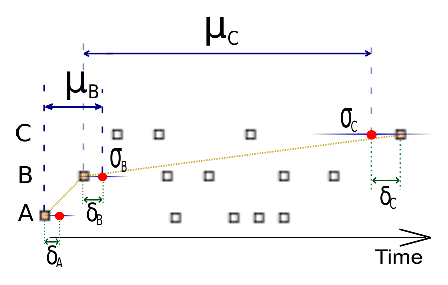
\includegraphics[scale=0.9]{il1.eps}
\end{center}

%\begin{left}
%\begin{tabular}[t]{p{12em}|p{12em}}
%    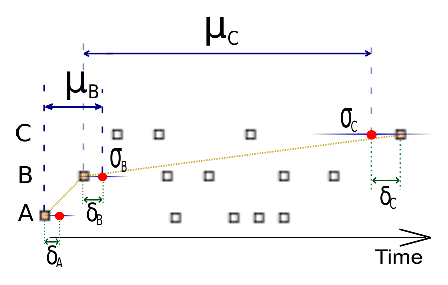
\includegraphics[scale=0.6]{il1.eps} & 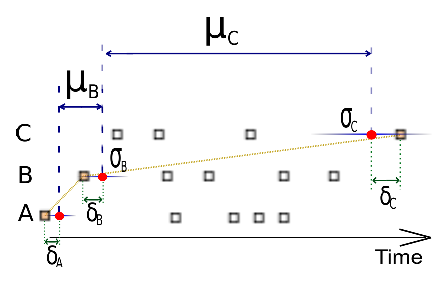
\includegraphics[scale=0.6]{il2.eps}\\
%\end{tabular}
%\end{left}
\end{frame}

\subsection{ Patterns construction }

\begin{frame}
  \frametitle{Loss function }
  \begin{itemize}
  \item Penalty for missing $x$ events in pattern of length $N$:
  $$
  f_{LOSS}(x,N)= \begin{cases}
   \exp\bigl(-\frac{\lambda x}{N}\bigr), & x < N, \\
   0,                                    & x=N.
   \end{cases}
  $$
  \item $\lambda$ defines level of pattern's fuzziness.
   \end{itemize}
   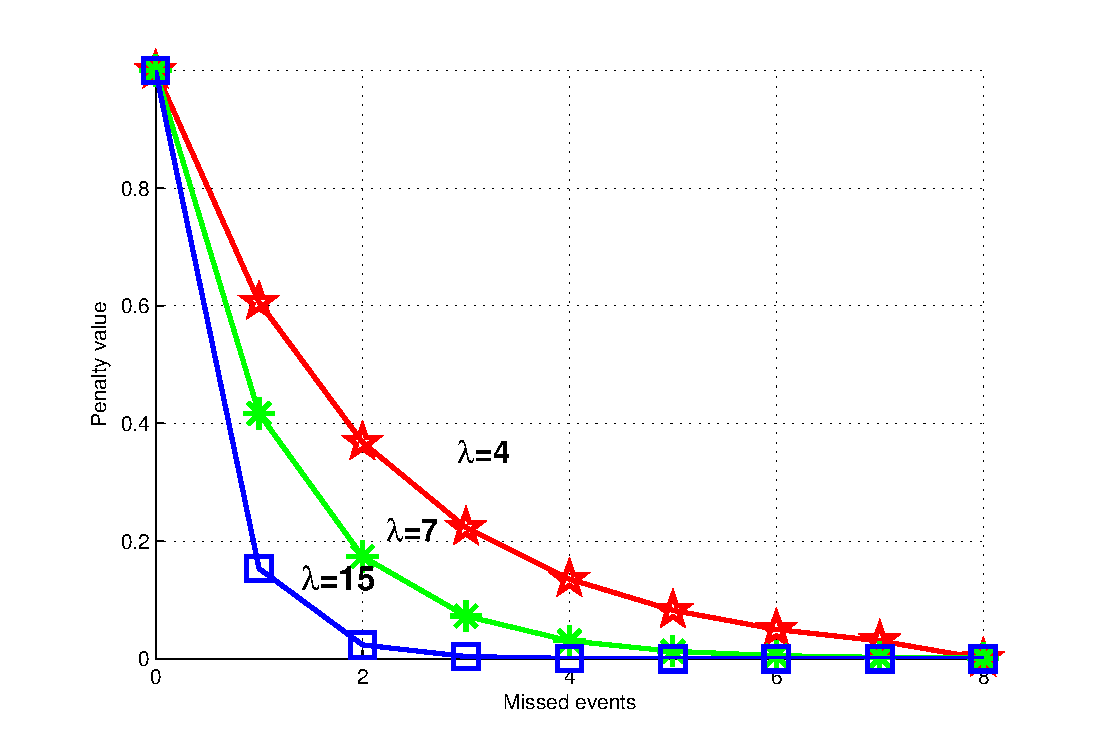
\includegraphics[scale=0.35]{MB_LF.eps}
\end{frame}

\begin{frame}
  \frametitle{Likelihood }
  For every pattern $P$ of length $N$, for every time moment $\varepsilon\in[0,N_t]$ 
  $$
  L_P(\varepsilon)=f_{LOSS}(N_-,N)\prod_{i=1}^{N}\biggl( \frac1{\sqrt{2\pi}\sigma_i }\biggr)  
  \prod_{i=1}^{N_+}\exp\biggl(- \frac{\delta_i^2}{2\sigma_i^2}\biggr)
  $$
  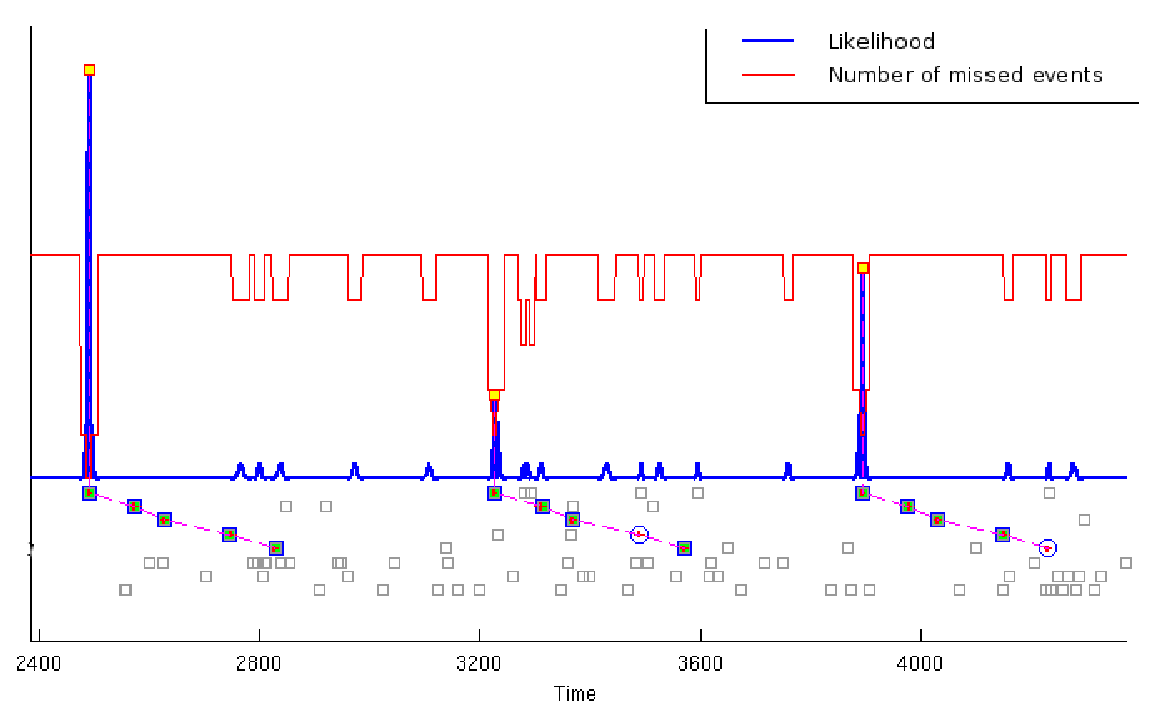
\includegraphics[scale=0.4]{norm_12_of_14.eps}
\end{frame}

\begin{frame}
  \frametitle{Detecting co-occurrences }
\begin{itemize}
  \item Computing distribution of distances between two patterns.
  \item Searching $\mu$ and $\sigma$, that fits that distribution.
  \item Determine, if there is a relation between patterns.
\end{itemize}
  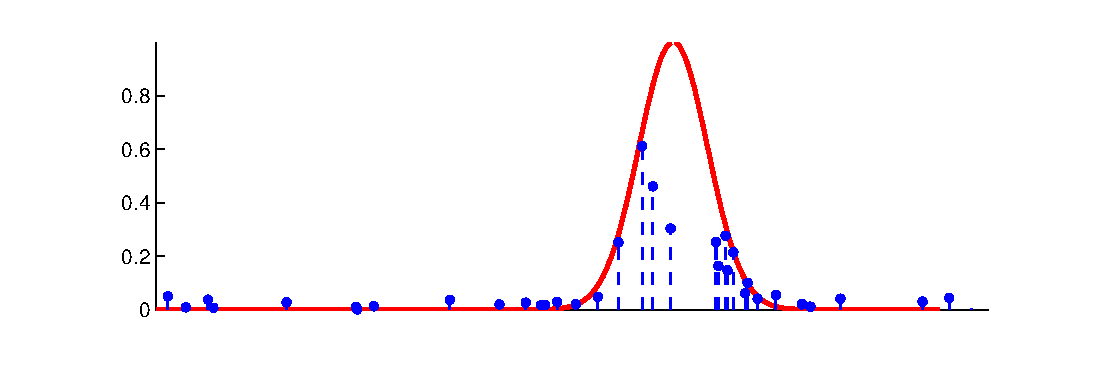
\includegraphics[scale=0.4]{weights.eps}
\end{frame}

\subsection{ Redundant patterns }
\begin{frame}
  \frametitle{Type of unnecessary patterns}
\begin{itemize}
  \item {\bf Duplicates: } $(AB)(CD), ((AB)C)D$.
  \item {\bf Incomplete copies: } $BCD$ doesn't occur outside of 
				  $ABCD$.
  \item Similarity of patterns, using likelihood vector $\overrightarrow{L}$. Correlation coefficient:
  $$
  cor(\overrightarrow{L_1}, \overrightarrow{L_2}) = \frac{\overrightarrow{L_1}\overrightarrow{L_2}^T}
  {\sqrt{\overrightarrow{L_1}\overrightarrow{L_1}^T}\sqrt{\overrightarrow{L_2}\overrightarrow{L_2}^T}}
  $$
\end{itemize}
\end{frame}

\begin{frame}
  \frametitle{ Elimination of patterns }
  Consider patterns $P_1$ and $P_2$.
  If $P_1$ consists of all events, that are met in $P_2$ and  
  $\exists m: cor(\overrightarrow{L_{P_1,1}}, \overrightarrow{L_{P_2,m}}) > \nu$, then
  $P_1$ is dropped.
\end{frame}

\subsection{ The method analysis }
\begin{frame}
  \frametitle{ Parameters of algorithm }
    
    \begin{tabular}{ |p{5em} | p{4em} | p{4em} | p{8em}| }
    
    \hline
    \bf{Parameter} & \bf{ Possible values} & \bf{ Default value} & \bf{ Has influence on } \\
    \hline
    \omega & $[0,1]$ & 0.995 & Significance of pattern \\ \hline
    \mu & $[0, +\infty]$ & 3 & Minimal pattern occurrences  \\ \hline \hline
	\mu & $[0, +\infty]$ & 6 & Fuzziness of patterns  \\  \hline    
    \nu & $[0,1]$ & 0.7 & Similarity of patterns for elimination \\ \hline
    $M$ & $[0,N_t]$ & None & Max time span between events in patterns \\ \hline
    \end{tabular}

\end{frame}

\begin{frame}
  \frametitle{ Experiments on real data }
  \begin{itemize}
  	\item
    Patterns found, using different methods:\\
    \begin{tabular}{ |p{6em} || p{9em} | p{6em}| }
    
    \hline
    \bf{T-Patterns} & \bf{ T-Patterns found, using Fuzzy patterns} & 
    \bf{ New fuzzy patterns}\\
    \hline \hline
    21 & 18 & 3 \\ \hline
    87 & 84 & 21 \\ \hline
    96 & 80 & 13 \\ \hline
    58 & 57 & 21 \\ \hline
    
    \end{tabular}
	\\ \\ \\
	\item
	Histogram of pattern's lengths:\\
	 \begin{tabular}{ |c| c c c c c c c | }
    \hline
    \bf{Pattern's length} & 2 & 3 & 4 & 5 & 6 & 7 & 8 \\ \hline\hline
    \bf{ T-Patterns} & 18 & 38 & 12 & 18 & 3 & 1 & 0 \\ \hline
    \bf{ Fuzzy patterns} & 22 & 41 & 14 & 20 & 6 & 4 & 2 \\ \hline
    
    \end{tabular}
   \end{itemize}
\end{frame}

\begin{frame}
  \frametitle{ Conclusion }
\begin{itemize}
  \item Longer and more complex patterns are found.
  \item Statistical roots.
  \item Computational complex.
\end{itemize} 
\end{frame}


\end{document}

